\documentclass[a4paper, 12pt]{book}

% ===== PACCHETTI NECESSARI ===== %
\usepackage[margin=2.5cm]{geometry}
\usepackage[italian]{babel}
%\usepackage{wrapfig}
\usepackage{graphicx}
\usepackage{hyperref}
\usepackage{subcaption}
\usepackage{amsmath}
\setlength{\parindent}{0pt}
\usepackage{parskip}
\usepackage[most]{tcolorbox}
\usepackage{soul}
\usepackage{xcolor}
\sethlcolor{yellow}
\usepackage{array}
\usepackage{booktabs}
\usepackage{tikz}
\usetikzlibrary{positioning}
\usepackage{longtable}
\usepackage{array}
\usepackage{fancyhdr}
\setlength{\headheight}{15pt}
\pagestyle{fancy}
\fancyhf{} % pulisce header e footer
\fancyhead[R]{\thepage} % numero pagina a destra nell'header
\renewcommand{\headrulewidth}{0pt} % (opzionale) elimina la riga orizzontale sotto l'header
\fancypagestyle{plain}{%
  \fancyhf{} % pulisce header e footer
  \fancyhead[R]{\thepage} % numero sempre in alto a destra
  \renewcommand{\headrulewidth}{0pt} % opzionale: niente linea
}
\setcounter{tocdepth}{3}


% ===== LISTA COMANDI =====
%------COMANDO DEFINIZIONE-------%
\newcommand{\definizione}[2]{%
  \vspace{15pt}%
  \begin{tcolorbox}[
    colback=cyan!5!white,
    colframe=blue!50!black,
    title=\textbf{Definizione - #1}, % titolo della definizione
    coltitle=white,
    fonttitle=\bfseries,
    arc=3mm,
    boxrule=0.5pt,
    enhanced,
    breakable
  ]
  #2 % testo della definizione
  \end{tcolorbox}
  \vspace{15pt}%
}


\title{\textbf{Elaborazione di segnali e immagini}}
\author{Mattia Nicolis \and Matteo Drago}
\date{A.A. 2025-26}

\begin{document}

    \maketitle

    \tableofcontents
    \markboth{}{}

    %-------MODULO DI TEORIA------------------------------------
    %-------Prof: Manuele Bicego--------------------------------
    %-------Lez: mercoledì (8:30-11:30) [Aula Delta - Cav.3]----
    \chapter*{Teoria}
    \addcontentsline{toc}{chapter}{Teoria}

    \section*{Sistemi e segnali}
    \addcontentsline{toc}{section}{Sistemi e segnali}

    \begin{figure}[h]
      \centering
      
\includegraphics[width=0.6\textwidth, keepaspectratio]{foto/sistemi&segnali.png}
      \caption{sistema e segnali}
    \end{figure}

    \definizione{segnale}{Un \textbf{segnale} è un \hl{insieme di dati o informazioni}.
    }


    Un segnale rappresenta qualsiasi tipo di variabile fisica soggetta a variazioni. 

    I segnali sono funzioni della variabile indipendente \textit{tempo} ($t$) o \textit{spazio} ($x, x = [x_1, x_2], x = [x_1, x_2, x_3]$).

    Sia la variabile indipendente che la variabile fisica possono essere scalari o vettoriali.

    Esempi di segnali:
    \begin{description}
      \item [segnali 1D]: segnale elettrocardiografico (EEG), segnale vocale, segnale audio
      \item [segnali 2D]: segnale immagine, segnale video 
      \item [segnali 3D]: segnale di dati volumetrici
    \end{description}

    \begin{figure}[h]
      \centering

      \begin{subfigure}[b]{0.45\textwidth}
        \centering
        
\includegraphics[width=\textwidth, height=3.8cm]{foto/segnale-audio.png}
        \caption{segnale 1D - segnale audio}
      \end{subfigure}
      \hfill
      \begin{subfigure}[b]{0.45\textwidth}
        \centering
        
\includegraphics[width=\textwidth, height=3.8cm]{foto/segnale-elettrocardiogramma.png}
        \caption{segnale 1D - elettrocardiogramma}
     \end{subfigure}
    \end{figure}

    \
    
    Un segnale può essere elaborato da un \textbf{sistema}.

    \definizione{Sistema}{Un \textbf{sistema} è un'\hl{entità che elabora un insieme di segnali (\textit{input}) per produrre un altro insieme di segnali (\textit{output})}.
    }

    I sistemi processano i segnali per:
    \begin{itemize}
      \item estrarre informazioni
      \item consentire la trasmissione su canali con capacità limitata (JPEG, JPEG2000, codifica MPEG)
      \item migliorare la sicurezza sulle reti (crittografia, watermarking)
      \item migliorare la sicurezza sulle reti (crittografia, watermarking)
    \end{itemize}

    \begin{figure}[h]
      \centering
      
\includegraphics[width=0.6\textwidth, keepaspectratio]{foto/sistema.png}
      \caption{sistema}
    \end{figure}

    La funzione che collega l'uscita del sistema con il segnale di ingresso è chiamata \textbf{risposta all'impulso} $h(t)$ nel dominio del \textit{tempo} e \textbf{funzione di trasferimento} $H(\omega)$ nel dominio della \textit{frequenza}. 

    \subsection*{Classificazione dei segnali}
    \addcontentsline{toc}{subsection}{Classificazione dei segnali}
    I segnali possono essere di 4 tipologie:
    \begin{itemize}
      \item \textbf{segnali a tempo continuo} e \textbf{a tempo discreto}
      \item \textbf{segnali analogici} e \textbf{digitali}
      \item \textbf{segnali periodici} e \textbf{aperiodici}
      \item \textbf{segnali energetici} e \textbf{segnali di potenza}
      \item \textbf{segnali deterministici} e \textbf{probabilistci}
    \end{itemize}

    \subsubsection*{Segnali a tempo continuo e a tempo discreto}
    \addcontentsline{toc}{subsubsection}{Segnali a tempo continuo e a tempo discreto}







    %-------MODULO DI LABORATORIO-------------------------------
    %-------Prof: Menegaz Gloria--------------------------------
    %-------Lez: giovedì (15:30-18:30) [Aula A - Cav.1]---------
    \chapter*{Laboratorio}
    \addcontentsline{toc}{chapter}{Laboratorio}

    \section*{Introduzione a Matlab}
    \addcontentsline{toc}{section}{Introduzione a Matlab}

    \subsection*{Layout di Matlab}
    \addcontentsline{toc}{subsection}{Layout di Matlab}
    \begin{figure}[h]
      \centering
      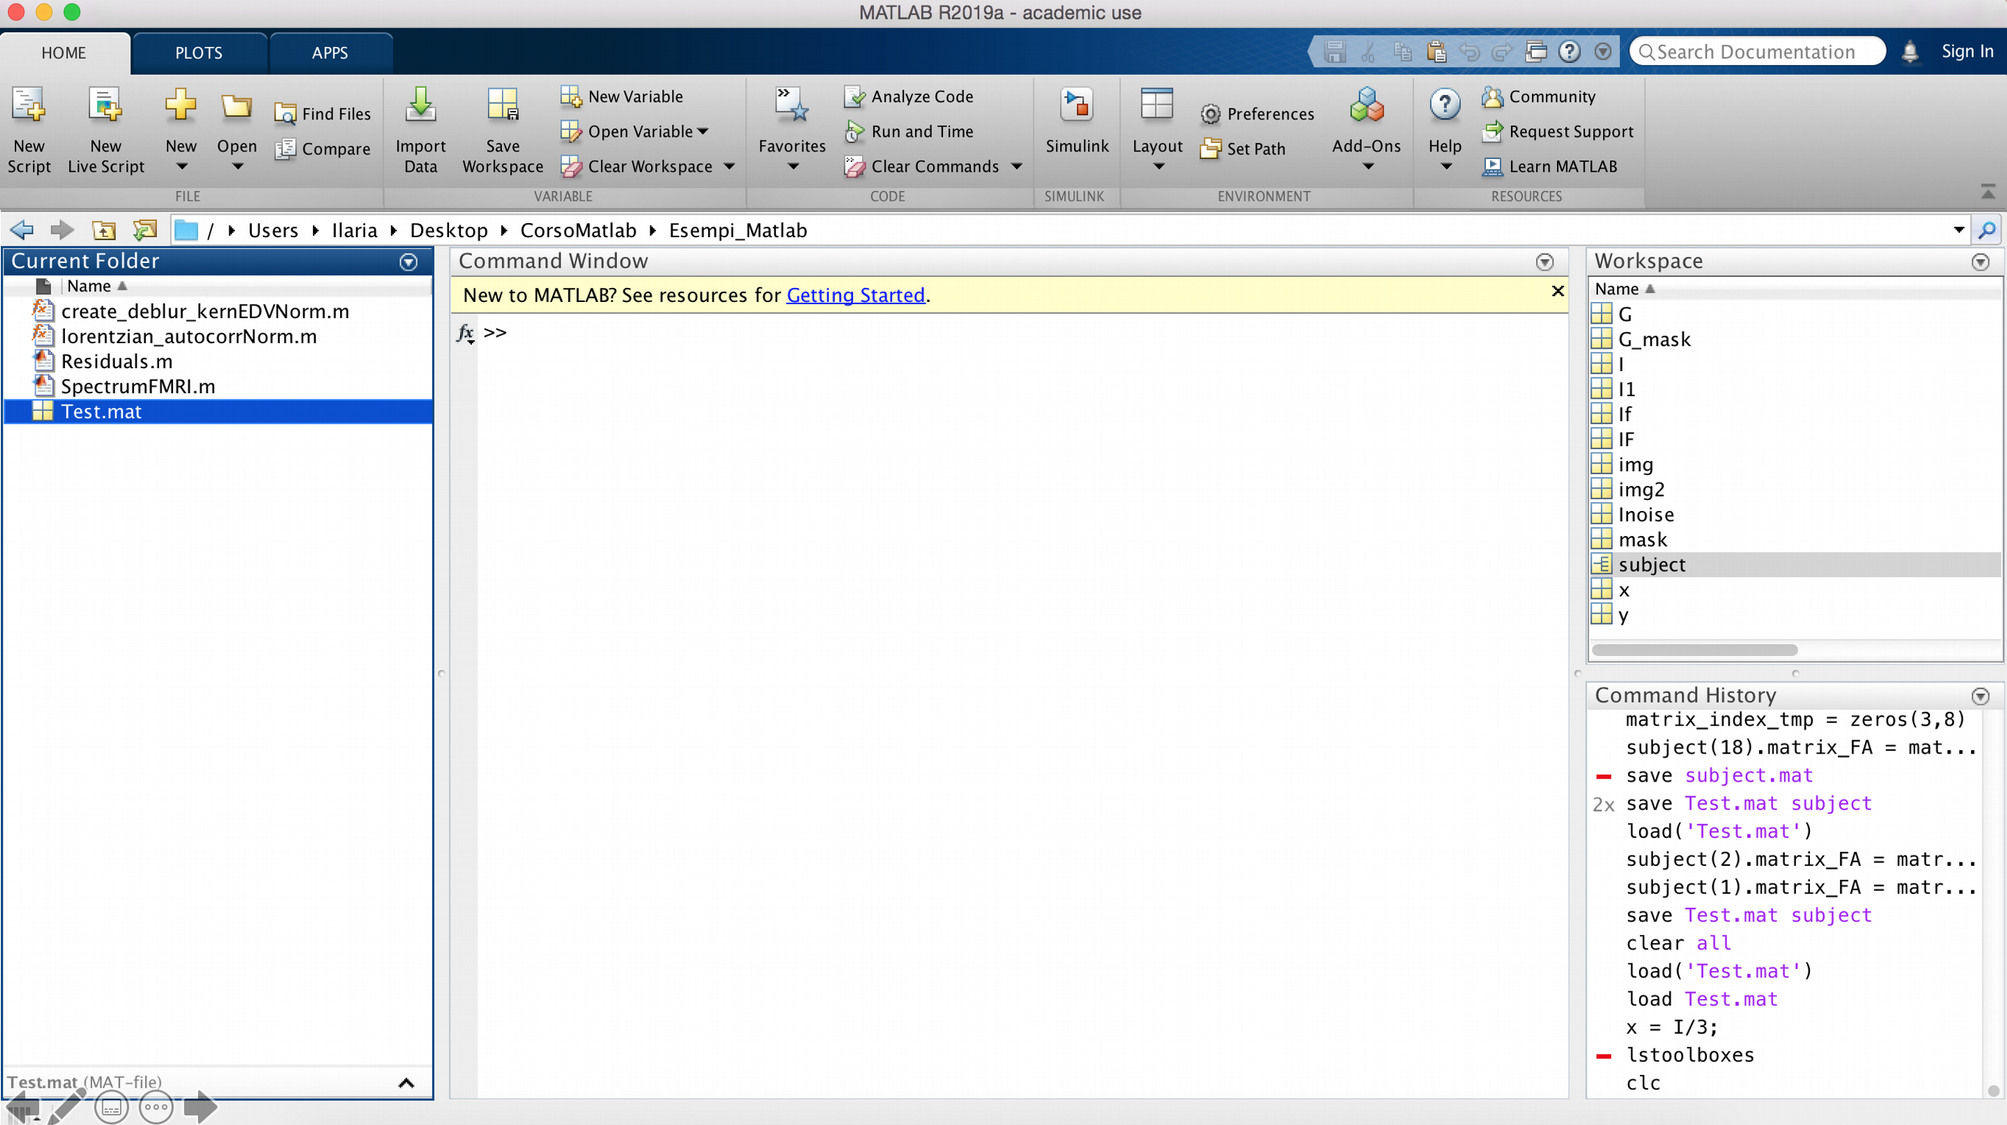
\includegraphics[width=0.8\textwidth, keepaspectratio]{foto/images-lab/layout.png}
      \caption{layout di Matlab}
    \end{figure}

    Il layout di Matlab è costituito da 4 sezioni principali:
    \begin{itemize}
      \item \textbf{Command Window}: finestra principale di interazione e contiene il comando prompt(\verb|>>|).
      
      E' la finestra che ci permette di interagire con Matlab: serve oer inserire comandi e stampare a video i risultati.

      \item \textbf{Command History}: visualizza una lista di comandi precendetemente digitati.
      
      La cronologia rimane per più sessione, i comandi possono essere caricati direttamente sulla command window ed eventualmente modificati oppure doppio click per rieseguirli

      \item \textbf{Workspace}: contiene la lista di tutte le variabili create durante la sessione di lavoro corrente, insieme alle loro informazioni principali
      \item \textbf{Current Folder}: mostra i file che sono contenuti nella cartella di lavoro corrente, anche suddivisi per tipologia
    \end{itemize}

    Matlab può essere utilizzato per eseguire calcoli di base (operazioni aritmetiche, esponenziali e numeri complessi) come una normale calcolatrice scientifica.

    \subsection*{Definizione di matrici e vettori}
    \addcontentsline{toc}{subsection}{Definizione di matrici e vettori}
    Matlab è un \hl{linguaggio di programmazione orientato alle matrici}.

    Gli \textbf{scalari} sono rappresentati come matrici $1 \times 1$.

    I \textbf{vettori} sono particolari metrici con una sola riga e n colonne (\textit{vettori riga}) o con una sola colonna e m righe (\textit{vettori colonna}).

    Matlab alloca utomaticamente le matrici in memoria pertanto non è necessario dichiararne le dimensioni prima di usarle.

    \begin{figure}[h]
      \centering
      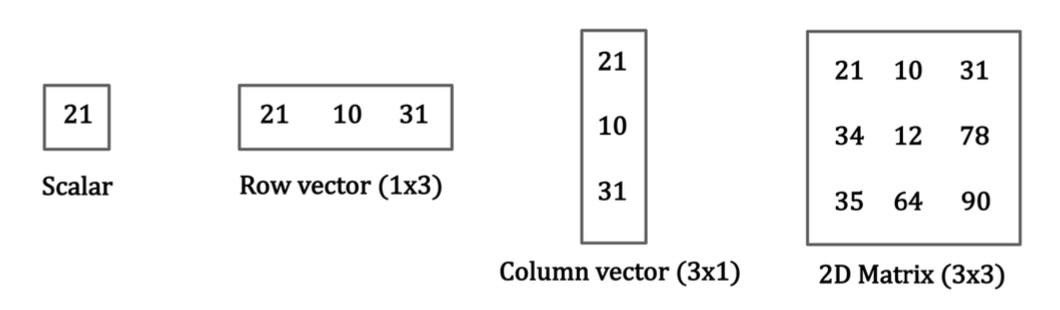
\includegraphics[width=0.6\textwidth, keepaspectratio]{foto/images-lab/matrici.png}
      \caption{tipologie di matrici in Matlab}
    \end{figure}

    Le matrici si inserisco come segue:
    \begin{itemize}
      \item gli elementi di una colonna sono separati da spazi o virgole
      \item le righe sono separate da punto e virgola (;)
      \item le matrici si racchiudono tra parentesi quadre []
    \end{itemize}

    %esempio: istruzione A = [1 2 3; 4 5 6; 7 8 9] risulato ....

    Per accedere agli elementi di una matrice si usano gli indici di riga e colonna racchiusi tra parentesi tonde ():
    \begin{description}
      \item [\texttt{>>} x(3)] restituisce il terzo elemento del vettore x
      \item [\texttt{>>} A(2,3)] restituisce l'elemento alla seconda riga e terza colonna della matrice A
      \item [\texttt{>>} A(1,:)] restituisce la seconda riga della matrice A
      \item [\texttt{>>} A(:,1)] restituisce la prima colonna della matrice A
      \item [\texttt{>>} A(2:3,1:2)] estrae una sottomatrice di A costituita dagli elementi delle righe 1 e 2 e delle colonne 2 e 3
    \end{description}

    Le matrici possono esser costruite a partire da matrici di dimensioni minori:
    \begin{description}
      \item [\texttt{>>} x(5) = abs(x(1))] produce x = [-1.3000 2.6667 4.8000 0 1.3000]
    \end{description}

    La dimensione di $x$ viene automaticamente incrementata per inglobare il nuovo elemento e gli elementi indefinti viene posto uguale a zero.

    Per creare un vettore di punti equispaziati si può usare l'istruzione x = [inizio:passo:fine]:
    \begin{description}
      \item [\texttt{>>} x = [1:4]] produce x = [1 2 3 4]
      \item [\texttt{>>} x = [1:3:8]] produce y = [1 4 7]
    \end{description}

    In alternativa si può usare l'istruzione \texttt{linspace(inizio, fine, num\_punti)}, se si vuole un vettore di numri linearmente spaziati, altrimenti il comando \texttt{logspace(inizio, fine, num\_punti)} per vettori con spaziatura logaritmica:
    \begin{description}
      \item [\texttt{>>} z = linspace(2,14,6)] produce z = [2.0000 4.4000 6.8000 9.2000 11.6000 14.0000]
      \item [\texttt{>>} k = logspace(1,2,7)] produce k = [10.0000 14.6780 21.5443 31.6228 46.4159 68.1292 100.0000]
    \end{description}

    In Matlab, sono implementate varie funzioni che permettono di definire in maniera semplice delle matrici particolari:
    \begin{description}
      \item [\texttt{>>} zeros(m,n)] crea una matrice m x n di zeri
      \item [\texttt{>>} ones(m,n)] crea una matrice m x n di uni
      \item [\texttt{>>} eye(n)] crea una matrice identità di dimensione n x n
      \item [\texttt{>>} rand(m,n)] crea una matrice m x n di numeri casuali uniformemente distribuiti nell'intervallo (0,1)
      \item [\texttt{>>} randn(m,n)] crea una matrice m x n di numeri casuali con distribuzione normale standard (media 0 e varianza 1)
      \item [\texttt{>>} diag(v)] crea una matrice diagonale con gli elementi del vettore v sulla diagonale principale
    \end{description}

    Per verificare la dimensione di una matrice o il numero di elementi inclusi, ci sono diverse funzioni:
    \begin{description}
      \item [\texttt{>>} size(A)] restituisce la dimensione della matrice A
      \item [\texttt{>>} length(A)] restituisce la lunghezza del vettore A
      \item [\texttt{>>} numel(A)] restituisce il numero totale di elementi della matrice A
    \end{description}

    \subsection*{Operazioni tra matrici}
    \addcontentsline{toc}{subsection}{Operazioni tra matrici}
    Le operazioni fondamentali tra matrici, che devono avere la stessa dimensione per poter essere eseguite, sono:
    \begin{description}
      \item [\texttt{+}] somma tra matrici
      \item [\texttt{-}] sottrazione tra matrici
      \item [\texttt{.*}] moltiplicazione elemento per elemento
      \item [\texttt{./}] divisione elemento per elemento
      \item [\texttt{.\^}] elevamento a potenza elemento per elemento
    \end{description}

    Per valutare un'operazione "termine a termine", come molteplicare ogni termine del vettore $A$ per ogni termine del vettore $B$, si usa l'operatore \texttt{.*}:
    \begin{description}
      \item [\texttt{>>} A = [1 3 2]]
      \item [\texttt{>>} B = [-1 2 1]]
      \item [\texttt{>>} C = A .* B] 
      \item [C = [-1 6 2]]
    \end{description}

    Lo stesso si applica anche ad altre operazioni come la divisione e l'elevamento a potenza.
    
    L'operazione di \textit{trasposizione} è eseguita con l'operatore \texttt{'}:
    \begin{description}
      \item [\texttt{>>} A = [1 2 3; 4 5 6]]
      \item [\texttt{>>} B = A'] 
      \item [B = [1 4; 2 5; 3 6]]
    \end{description}

    Altre operazioni tra matrici imporatanti sono:
    \begin{description}
      \item [\texttt{>>} inv(A)] calcolo dell'inversa della matrice A (quadrata)
      \item [\texttt{>>} det(A)] calcolo del determinante della matrice A (quadrata)
      \item [\texttt{>>} diag(A)] estrae la diagonale principale della matrice A come vettore
      \item [\texttt{>>} trace(A)] calcola la somma degli elementi della diagonale principale della matrice A (quadrata)
      \item [\texttt{>>} eig(A)] calcola gli autovalori e gli autovettori della matrice A (quadrata)
      \item [\texttt{>>} rank(A)] calcola il rango della matrice A
      \item [\texttt{>>} norm(A)] calcola la norma della matrice A
      \item [\texttt{>>} sum(A)] calcola la somma degli elementi di ogni colonna della matrice A
      \item [\texttt{>>} prod(A)] calcola il prodotto degli elementi di ogni colonna della matrice A
      \item [\texttt{>>} min(A)] calcola il minimo degli elementi di ogni colonna della matrice A
      \item [\texttt{>>} max(A)] calcola il massimo degli elementi di ogni colonna della matrice A
      \item [\texttt{>>} mean(A)] calcola la media degli elementi di ogni colonna della matrice A
    \end{description}

    \subsection*{Comandi utili e istruzioni dos-like}
    \addcontentsline{toc}{subsection}{Comandi utili e istruzioni dos-like}
    In Matlab, ci sono una serie di funzioni di base che possono essere d'aiuto nella programmazione:
    \begin{description}
      \item [\texttt{>>} clc] pulisce la Command Window
      \item [\texttt{>>} dir] elenca i file nella cartella corrente
      \item [\texttt{>>} pwd] mostra il percorso della cartella corrente
    \end{description}

    Altre istruzioni utili sono:
    \begin{description}
      \item [\texttt{>>} type filename] visualizza il contenuto del file filename.m
      \item [\texttt{>>} delete filename] elimina il file filename.m
      \item [\texttt{>>} save filename] salva le variabili del workspace nella cartella corrente nel file filename.mat
      \item [\texttt{>>} load filename] carica le variabili dal file filename.mat nel workspace
      \item [\texttt{>>} ! command] esegue il comando di sistema command (es. \texttt{!dir} elenca i file nella cartella corrente)
      \item [\texttt{>>} $\uparrow$] richiama l'ultimo comando eseguito nella Command Window
    \end{description}
    
    Inoltre, per ottenere aiuto su una funzione o un comando specifico, si può utilizzare:
    \begin{description}
      \item [\texttt{>>} help functionname] visualizza la documentazione della funzione functionname
      \item [\texttt{>>} doc functionname] apre la documentazione completa della funzione functionname in una finestra separata
      \item [\texttt{>>} lookfor keyword] cerca la keyword nella documentazione di tutte le funzioni di Matlab
    \end{description}

    \subsection*{Script e function}
    \addcontentsline{toc}{subsection}{Script e function}
    Invece di inserire comandi direttamente nella Command Window, è possibile creare dei file di testo chiamati \textbf{script} o \textbf{function} che contengono una serie di comandi Matlab (estensione \texttt{.m}).

    Gli \textit{script file} contengono una serie di comandi Matlab che vengono eseguiti in sequenza quando lo script viene richiamato. 
    
    Gli script condividono lo stesso workspace della Command Window, quindi possono accedere e modificare le variabili definite nella Command Window.

    \

    Le \textit{function file} sono simili agli script, ma hanno una struttura più formale. 
    
    Le variabili vengono passate per valore, quindi contengono vari comandi che necessitano di variabili di input per essere eseguiti e producono variabili di output:
    \begin{center}
      \begin{verbatim}
        function [output] = functionName(input)
            % Corpo della function
        end
      \end{verbatim} 
    \end{center}
    
    Le variabili definite all'interno di una function sono locali a quella function e non influenzano il workspace della Command Window.
    
    Esempio di function che calcola una gaussiana:
    \begin{center}
      \begin{verbatim}
        function g1 = guassian(alpha, t)
            g1 = exp(-alpha*t.^2);
            ... command
        end
      \end{verbatim}
    \end{center}

    I commenti in Matlab iniziano con il "\%" e durano fino a afine della riga.

    Un doppio commento ha un significato particolare: delimita l'inizio di un blocco di codice che può essere eseguito singolarmente all'interno di uno script o di una function.

    E' una caratteristica utile per testare porzioni di codice senza dover eseguire l'intero script o function.

    \subsection*{Istruzioni di controllo}
    \addcontentsline{toc}{subsection}{Istruzioni di controllo}
    Tra le istruzioni di controllo che ci possono essere utili in Matlab
    \begin{description}
      \item [\texttt{if ... elseif ... else ... end}]: istruzione condizionale
        \begin{verbatim}
          if condizione1
              ... comandi se condizione1 è vera
          elseif condizione2
              ... comandi se condizione2 è vera
          else
              ... comandi se nessuna condizione è vera
          end
        \end{verbatim}

      \item [\texttt{for ... end}]: ciclo for
        \begin{verbatim}
          for indice = inizio:passo:fine
              ... comandi da eseguire in ogni iterazione
          end
        \end{verbatim}

      \item [\texttt{while ... end}]: ciclo while
        \begin{verbatim}
          while condizione
              ... comandi da eseguire finché la condizione è vera
          end
        \end{verbatim}
    \end{description}
    
    Gli operatori logici principali in Matlab sono:
    \begin{description}
      \item [\texttt{\&}]: operatore AND logico
      \item [\texttt{|}]: operatore OR logico
      \item [\texttt{~}]: operatore NOT logico
      \item [\texttt{xor}]: operatore XOR logico
    \end{description}

    Gli operatori relazionali principali in Matlab sono:
    \begin{description}
      \item [\texttt{==}]: uguale a
      \item [\texttt{~=}]: diverso da
      \item [\texttt{>}]: maggiore di
      \item [\texttt{<}]: minore di
      \item [\texttt{>=}]: maggiore o uguale a
      \item [\texttt{<=}]: minore o uguale a
    \end{description}
\end{document}